\documentclass{ximera}

\input{../preamble.tex}


\title{Fractions and decimals}
\author{Jenny Sheldon}

\begin{document}

\begin{abstract}
We connect ideas we've discussed separately.
\end{abstract}
\maketitle

\section{Activities for this section:} 
\link[Work On Wording]{https://ximera.osu.edu/m4t/elementaryActivities/SemesterOnePacket/elementaryActivities/Numbers/WorkOnWording}




\section{Fractions and decimals}

You might have noticed  that we use the same language to describe $\frac{1}{10}$ and $0.1$. Both of them are called ``one tenth'', but we have defined them differently. Let's see how these ideas are actually the same thing.

\begin{example}
Explain why $\frac{1}{10}$ and $0.1$ are the same value. 

We will start by drawing a whole which also has the value $1$.
\begin{image}
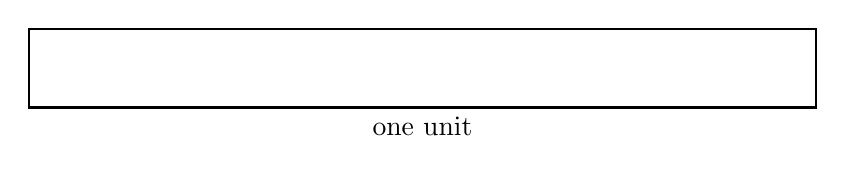
\begin{tikzpicture}
\draw[thick] (0,0) rectangle (10,1);
\node[below] at (5,0) {one unit};
\end{tikzpicture}
\end{image}

To find $\frac{1}{10}$ of this whole, we need to cut it into $\answer[given]{10}$ equal pieces, based on the meaning of the denominator, and then shade $\answer[given]{1}$ piece, based on the meaning of the numerator. Let's do that in our picture.
\begin{image}
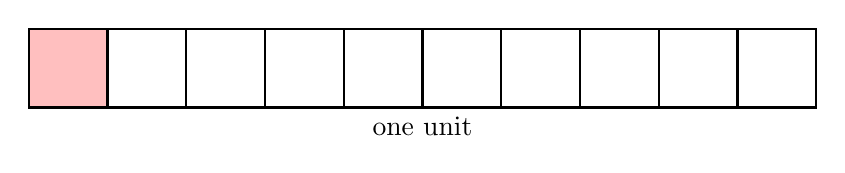
\begin{tikzpicture}
\draw[fill=pink] (0,0) rectangle (1,1);
\draw[thick] (0,0) rectangle (10,1);
\node[below] at (5,0) {one unit};
\foreach \x in {1, 2, ..., 9} \draw[thick] (\x, 0)--(\x, 1);
\end{tikzpicture}
\end{image}
Using our definition of fractions, this shaded piece is $\frac{1}{10}$ of the whole. But what if we thought about this using bundling? We started with one unit, and then unbundled it into $\answer[given]{10}$ equal sections. By definition, each section has the value $\answer[given]{0.1}$ because when we unbundle, we move exactly one place value right.

In other words, this shaded region is $\frac{1}{10}$ of the unit, and its value is also $0.1$. Since it's the same shaded region, these values must be equal.
\[
\frac{1}{10} = 0.1
\]
\end{example}

Similarly, we could unbundle each of the $0.1$-sized pieces, meaning that the new, smaller pieces would each have the value $0.01$. Unbundling each of the $10$ equal pieces into $10$ more equal pieces would mean that our whole is split into $100$ equal pieces, or that each piece is worth $\frac{1}{100}$. In this way we can see that 
\[
\frac{1}{100} = 0.01.
\]
This process could continue as long as we like. 
\begin{question}
Using thinking like we just described, what are the decimal values of the fractions below?

\begin{itemize}
	\item $\frac{1}{1000} = \answer{0.001}$
	\item $\frac{1}{10000} = \answer{0.0001}$
	\item $\frac{1}{100000} = \answer{0.00001}$
\end{itemize}
\end{question}

We can use this connection between fractions and decimals to write other fractions as decimals as well.

\begin{example}
Write $\frac{9}{20}$ as a decimal. 

Since we want to use one of the facts above, we want to change this fraction into an equivalent fraction whose denominator is $10$, $100$, $1000$, or some other power of $10$. We know that $20 \times \answer[given]{5} = 100$, so we can make an equivalent fraction with denominator $100$ in this case. We have
\[
\frac{9}{20} = \frac{\answer[given]{45}}{100}.
\]
Now, we know that $\frac{1}{100} = \answer[given]{0.01}$ as a decimal, and that according to our meaning of fractions $\frac{45}{100}$ is $45$ pieces, each of size $\frac{1}{100}$. This means that $\frac{45}{100}$ is also $45$ pieces, each of size $\answer[given]{0.01}$ as a decimal. We can think about this as $45$ individual blocks, each of value $0.01$. These $45$ blocks could be organized into $\answer[given]{4}$ bundles and $\answer[given]{5}$ individual blocks, and so the total value of all of these blocks would be $\answer[given]{0.45}$. In other words, 
\[
\frac{9}{20} = 0.45
\]
as a decimal.
\end{example}

The previous example shows us that if we can make an equivalent fraction whose denominator is a power of $10$ (like $10$, $100$, $1000$, etc), we can write the fraction as a decimal by looking at the numerator of that fraction. %Decimals like this one, which can be written as a fraction whose denominator is a power of $10$ and whose decimal values stop at some place value, are called \dfn{terminating decimals}. 

\begin{question}
Using the strategy of the example above, what is the decimal equivalent of the fraction $\frac{5}{8}$?

\begin{prompt}
$\answer{0.625}$
\end{prompt}
\end{question}


\begin{question}
Using a strategy similar to the one above, how would you write the decimal $0.735$ as a fraction?

\begin{prompt}
$\frac{\answer{735}}{1000}$
\end{prompt}
\end{question}








\end{document}






